\def\layersep{2.5cm}


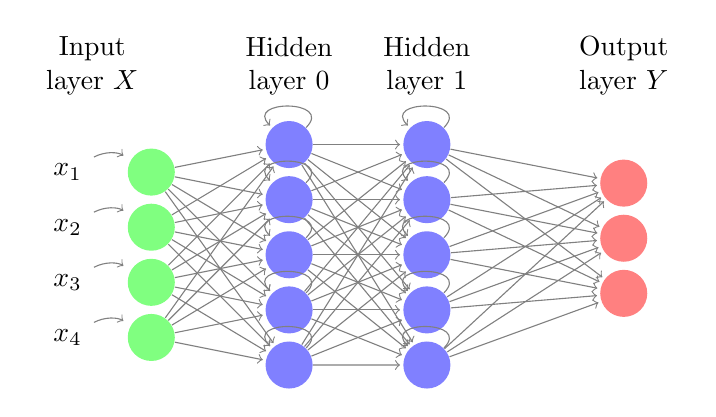
\begin{tikzpicture}[shorten >=1pt,->,draw=black!50, node distance=\layersep, scale = 0.7]
    \tikzstyle{every pin edge}=[<-,shorten <=3pt, bend right]
    \tikzstyle{neuron}=[circle,fill=black!25,minimum size=17pt,inner sep=0pt]
    \tikzstyle{input neuron}=[neuron, fill=green!50];
    \tikzstyle{output neuron}=[neuron, fill=red!50];
    \tikzstyle{hidden neuron}=[neuron, fill=blue!50];
    \tikzstyle{annot} = [text width=4em, text centered]
    
    \tikzset{every loop/.style={min distance=3mm,looseness=3}}
    
    %\node at (0,-2) {$\vdots$};

    % Draw the input layer nodes
    \foreach \name / \x in {1,...,4} {
    % This is the same as writing \foreach \name / \y in {1/1,2/2,3/3,4/4}
    	\pgfmathparse{\x<5 ? \x : "n"}
        \node[input neuron, pin=left:$x_{\pgfmathresult}$] (I-\name) at (0,-\x) {};
        
    }

    % Draw the hidden layer nodes
    \foreach \name / \y in {1,...,5}
        \path[yshift=0.5cm]
            node[hidden neuron] (H-\name) at (\layersep,-\y cm) {};
            
    % Draw the hidden layer nodes
    \foreach \name / \y in {1,...,5}
        \path[yshift=0.5cm]
            node[hidden neuron] (H2-\name) at (\layersep*2,-\y cm) {};

    
    \foreach \name / \y in {1,...,3}
        \path[yshift=-0.2cm]
            node[output neuron,right of=H2-1] (O-\name) at (\layersep*2,-\y cm) {};

    % Connect every node in the input layer with every node in the
    % hidden layer.
    \foreach \source in {1,...,4}
        \foreach \dest in {1,...,5}
            \path (I-\source) edge (H-\dest);
            
    \foreach \source in {1,...,5}
        \foreach \dest in {1,...,5}
            \path (H-\source) edge (H2-\dest);


	
    \foreach \source in {1,...,5}
            \path(H-\source) edge[loop] (H-\source);
            
    
    \foreach \source in {1,...,5}
            \path(H2-\source) edge[loop] (H2-\source);

        
    \foreach \source in {1,...,5}
        \foreach \dest in {1,...,3}
            \path (H2-\source) edge (O-\dest);

    % Annotate the layers
    \node[annot,above of=H-1, node distance=1cm] (hl) {Hidden layer 0};
    \node[annot,above of=H2-1, node distance=1cm] (hl2) {Hidden layer 1};
    \node[annot,left of=hl] {Input layer $X$};
    \node[annot,right of=hl2] {Output layer $Y$};
\end{tikzpicture}